PocketShelf is an inventory IOS/Android application. Our application consist of many features among which adding item/shelf, search item for each user with Augmented reality experience is the key feature of our application. Diagram below show the overall high level feature of our application.


\begin{figure}[h!]
	\centering
 	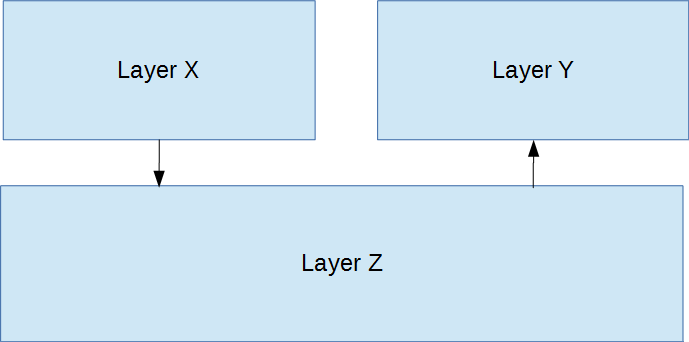
\includegraphics[width=0.60\textwidth]{images/layers}
 \caption{A simple architectural layer diagram}
\end{figure}

\subsection{SignUp}
This is the initial step that is needed to to taken by the user. This layer allows user to create the new account once clicked to signUp in L/R\_UI. In this layer user are required to input the username, email and strong alpha-numeric password. Before any execution the input of the user is validated. Once input is validated, this layer will send the verification to the provided email. If the validation and verification is successful, new user is created and all user information is recorded to our database and user is redirected to L/R\_UI.

\subsection{LogIn}
If user clicks LogIn in L/R\_UI, user is redirected to this layer. This layer allow the existing User to login to their account. This layer user to input username and password. Similarly username and password is validated prior to any execution to any query. If valid input are given, layer will logged the user to their respective user home\_UI, if user are registered prior to login.

\subsection{AddItem}
Once user is Logged in to the system, this layer will allow user to add item to the inventory. User are required to provide the item description, after which all the input are validated prior to use for any queries. All the valid input are sent to QR\_Generator, where QR is created for the item, QR\_Generator will send the QR image along with item description to DB\_Controller, where DB\_Controller will find the spot to keep. Once spot is assigned it will return the the QR image and Shelf information to Display\_UI. Which will display the information of the shelf, where it is added along with item description. 

\subsection{AddShelf}
Logged user have the option to add the customized shelf. This layer will allow user to input the shelf description, which is first validated then the valid shelf description is passed to the DB\_Controller, which will save and update the available spot for adding item in the application. After adding to the inventory DB\_Controller will return the number of Spot added to Dispaly\_UI. This will display descriptive added shelf to the user.

\subsection{Search}
Search is one of the core feature of our application. User are able to search any item in the inventory based on the entered text or the QR code that is generated during adding shelf. Once the application gets the user input, it looks up on the Database, then the application pulls the image of the item on the shelf, if the item is what user is looking for s/he clicks confirm which is then shown to user via Search\_UI.

\subsection{Home\_UI}
Home\_UI is the graphic feature of the application. It is responsible for generating necessary UI shown to the user. Once user logged in to his/her account, application will redirect them to Home\_UI, from where they can toggle between 